\chapter{Réalisations de la pointeuse}
\fancyhead[R]{\textit{Réalisations et programmation de la pointeuse}}
\renewcommand{\headrulewidth}{1pt}

\section{Introduction}
Dans ce chapitre, nous aborderons l’aspect matériel du projet ; en l’occurrence 
la pointeuse biométrique à réaliser. En premier lieu, nous allons décrire 
Arduino en tant que plateforme, puis nous décrirons en détail le microcontrôleur 
choisi en justifiant le choix de ce dernier. Par la suite, nous citerons les 
caractéristiques du capteur d’empreinte. Une fois assemblés, ils formeront notre 
dispositif de pointage. Nous exposerons les différents schémas de branchement et 
réaliserons un prototype en 3D pour avoir un aperçu de l’équipement à concevoir. 

La dernière section de ce chapitre concerne la communication entre la pointeuse 
et le système de gestions de pointage.

\section{Arduino}
Arduino est la marque d’une plateforme de prototypage open source, elle permet 
aux utilisateurs de créer des objets électroniques interactifs à partir de 
cartes électroniques matériellement libres sur lesquelles se trouve un 
microcontrôleur (d’architecture Atmel AVR. comme l’Atmega328p, et d’architecture 
ARM comme le Cortex-M3 pour l’Arduino due).

Les schémas de ces cartes électroniques sont publiés en licence libre. 
Cependant, certaines composantes, comme le microcontrôleur par exemple, ne 
sont pas sous licence libre. Le microcontrôleur peut être programmé pour 
analyser et produire des signaux électriques, de manière à effectuer des 
tâches très diverses comme la domotique (le contrôle des appareils 
domestiques — éclairage, chauffage…), le pilotage d’un robot, de l’informatique 
embarquée, etc. Arduino peut être utilisé pour construire des objets 
interactifs indépendants (prototypage rapide), ou bien peut être connecté à un 
ordinateur pour communiquer avec ses logiciels (ex.: Max/MSP, Usine Hollyhock, 
pure Data, SuperCollider).

\subsection{Matériel}
Un module Arduino est généralement construit autour d’un microcontrôleur Atmel 
AVR. (ATmega328, ATmega32u4 ou ATmega2560 pour les versions récentes, ATmega168, 
ATmega1280 ou ATmega8 pour les plus anciennes), et de composants complémentaires 
qui facilitent la programmation et l’interfaçage avec d’autres circuits. 
Le microcontrôleur est préprogrammé avec un Bootloader, de telle sorte qu’un 
programmateur dédié ne soit pas nécessaire. Les modules sont programmés avec 
une connexion série TTL, mais les connexions permettant cette programmation 
diffèrent selon les modèles. Les premiers Arduino possédaient un port série 
RS-232, puis l’USB est apparu sur les modèles Diecimila, tandis que certains 
modules destinés à une utilisation portable comme le Lillypad ou le promini se 
sont affranchis de l’interface de programmation, relocalisée sur un module 
USB-série dédié (sous forme de carte ou de câble). Des modules d’extension 
ont été conçus de sorte s’empiler sur l’Arduino. Plusieurs sortes d’extensions
sont disponibles dans le commerce.

Plusieurs cartes compatibles Arduino ont été produites par d’autres fabricants. 
Il existe aussi des cartes Arduino ou compatibles modifiés pour un usage 
spécifique: par exemple, des cartes de contrôle pour imprimantes 3D RepRap20, 
des systèmes de pilote automatique pour drones comme les systèmes ArduPilot, 
APM: Plane et APM:Copter, ou les cartes FlyDuino21, enfin des puces Wi-Fi 
tierces comme l’ESP8266 compatible avec l’environnement Arduino22.\cite{30}

\subsection{Logiciel}
Le logiciel de programmation des modules Arduino, dont l’interface est appelée 
Arduino IDE, est une application Java libre et multiplateforme dérivée de 
Processing servant d’éditeur de code et de compilateur, et qui peut transférer 
le firmware et le programme au travers de la liaison série (RS-232, Bluetooth 
ou USB selon le module). Il est également possible de se passer de l’interface 
Arduino, et de compiler et téléverser les programmes via l’interface en ligne 
de commande. Le langage de programmation utilisé est le C++, compilé avec 
avr.-g++ 8, et lié à la bibliothèque de développement Arduino, permettant 
d’utiliser la carte et ses entrées/sorties. La mise en place de ce langage 
standard rend aisé le développement de programmes sur les plateformes Arduino à 
toute personne maîtrisant le C ou le C++.\cite{31}

\section{ESP32}
ESP32 est une série de microcontrôleurs de type système sur une puce (SoC)
d’\emph{Espressif Systems}, basé sur l’architecture Xtensa LX6 de Tensilica
(en), intégrant la gestion du Wi-Fi et du Bluetooth (jusqu’à LE 5.0 et 5.11) en
mode double, et un DSP. C’est une évolution d’ESP8266. Son support Wi-Fi et
Bluetooth, en fait un système apprécié dans le domaine de l’internet des objets.
Ce SoC rencontre un certain succès depuis quelques années à la fois pour son
coût, ses capacités et son intégration dans un nombre croissant de
systèmes.\cite{32}

\begin{figure}[h!]
    \centering
    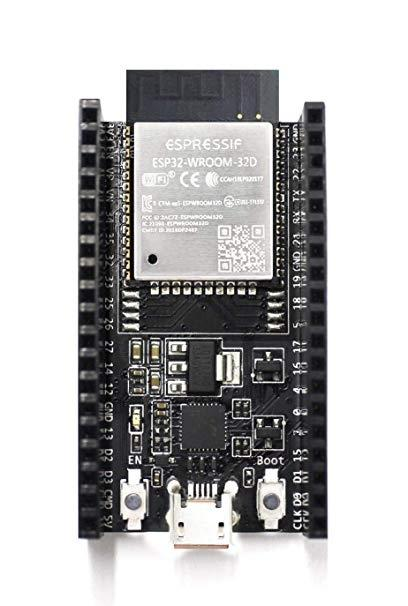
\includegraphics[scale=0.30]{images/esp32.jpg}
    \caption{ESP32 DevKit}
    \label{fig49}
\end{figure}

\subsection{Caractéristiques techniques}\cite{33}

\begin{itemize}
    \item[\textbullet]\textbf{Processeurs:}
        \begin{itemize}
            \item CPU: Xtensa double-cœur (ou simple-cœur), microprocesseur LX
                32 bits, fonctionnant à 160 ou 240 MHz et fournissant jusqu'à
                600 DMIPS ;

            \item coprocesseur ultra basse consommation (ULP) ;
        \end{itemize}

    \item[\textbullet]\textbf{Mémoire:} 520 KiO SRAM ;

    \item[\textbullet]\textbf{Connectivité sans-fil:}
        \begin{itemize}
            \item Wi-Fi: 802.11 b/g/n ;

            \item Bluetooth: v 4.2 BR/EDR et BLE jusqu'à v 5.0 et v 5.1 ;
        \end{itemize}

    \item[\textbullet]\textbf{Interfaces de périphériques}
        \begin{itemize}
            \item 12-bit Segmentation sur les ADC (SAR ADC) jusqu'à 18 canaux ;
            \item 2 × 8 bit DAC ;
            \item 10 × capteurs de touché (GPIO de capteur capacitif (en)) ;
            \item 4 × SPI ;
            \item 2 × interfacs I²S ;
            \item 2 × interfaces I²C ;
            \item 3 × UART ;
            \item contrôleur hôte SD/SDIO/CE-ATA (en)/MMC/eMMC ;
            \item contrôleur esclave SDIO/SPI ;
            \item interface MAC Ethernet avec DMA dédié et support du protocole
                de temps précis IEEE 1588 ;
            \item Bus de données CAN 2.0 ;
            \item contrôleur infrarouge distant (TX/RX, jusqu'à 8 canaux) ;
            \item Moteur PWM ;
            \item LED PWM (jusqu'à 16 canaux) ;
            \item Capteur à effet Hall ;
            \item préamplificateur analogique ultra-basse consommation ;
        \end{itemize}

    \item[\textbullet]\textbf{Sécurité}   
        \begin{itemize}
            \item Standard de sécurité supportant complètement IEEE
                802.11,incluant WPA/WPA2 et WAPI de WFA ;
            \item Secure boot (démarrage sécurisé) ;
            \item Chiffrement de la Flash ;
            \item 1024-bit OTP, jusqu'à 768 bits pour les clients
            \item Accélération matérielle du chiffrement: AES, SHA-2, RSA,
                elliptic curve cryptography (ECC), générateur de nombre
                aléatoire (en) (RNG) ;
        \end{itemize}
    \item[\textbullet]\textbf{Gestion de l'énergie}

        \begin{itemize}
            \item low-dropout regulator (en) interne;
            \item Domaines d'alimentation individuels pour le RTC;
            \item Alimentation en sommeil profond de 5 μA ;
            \item Réveil depuis des interruptions GPIO, timer, mesure ADC,
                interruption du capteur de touché capacitif.
        \end{itemize}
\end{itemize}


\begin{figure}[h!]
    \centering
    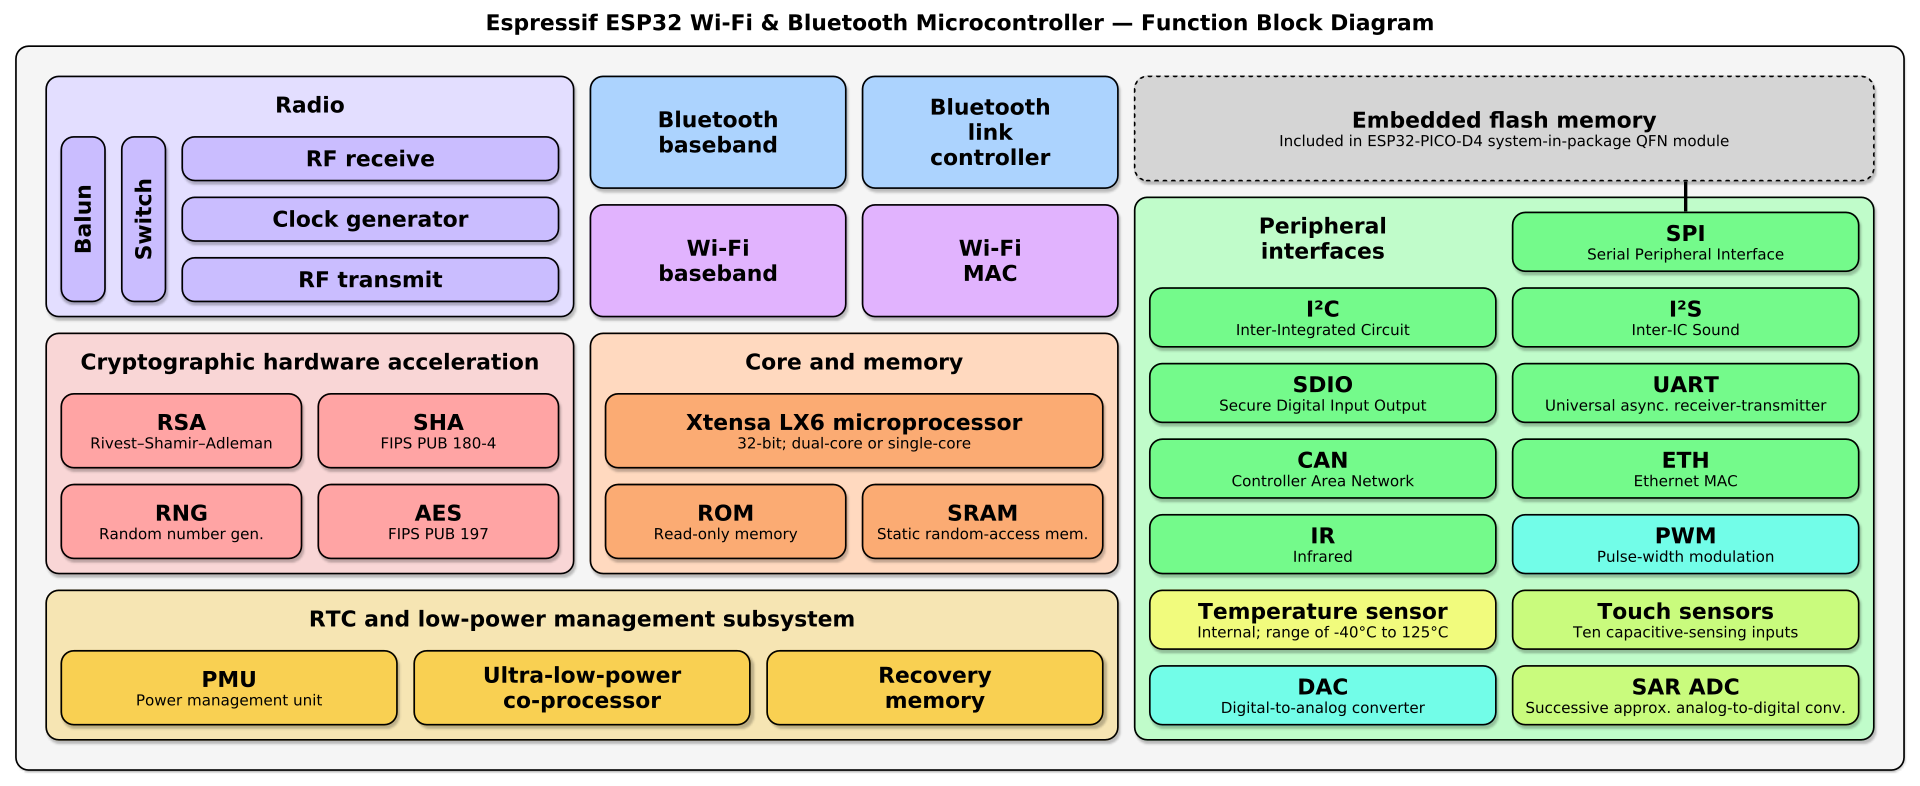
\includegraphics[scale=0.26 ]{images/esp32_fun.png}
    \caption{Schéma fonctionnel}
    \label{fig50}
\end{figure}

Le choix du module ESP32 Devkit est justifié par sa petite taille 
(57mm*28mm*3m), ainsi que ses caractéristiques techniques, notamment les
connectivités sans-fil, la sécurité, et la gestion de l’énergie.

\section{Capteur d'empreinte DY 50}
Les techniques utilisées pour capter les images des empreintes digitales sont 
diverses, d’où l’existence de plusieurs types de capteurs. L'on peut citer:

\begin{itemize}
    \item les capteurs thermique.
    \item les capteurs en silicium.
    \item les capteurs ultrasonique.
    \item les capteurs capacitif.
    \item les capteurs à champ électrique.
    \item les capteurs à pression.
    \item les capteurs optique.
\end{itemize}

Pour les besoins de notre projet, nous avons choisi le capteur DY50 de type
optique en raison de son coût, sa taille, et du fait d’avoir une image précise
de l’empreinte tout en étant intrinsèquement protégé contre les décharges
électrostatiques.

\begin{figure}[h!]
    \centering
    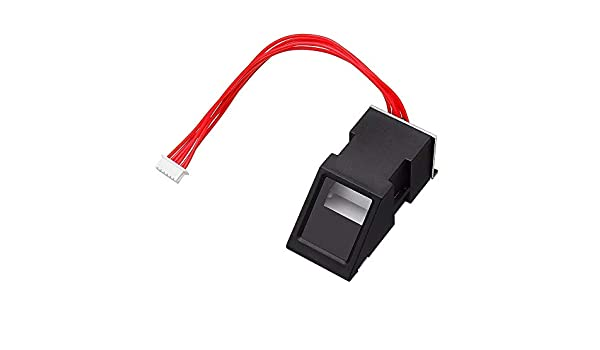
\includegraphics[scale=0.8]{images/dy50.jpg}
    \caption{Capteur optique DY50}
    \label{fig51}
\end{figure}

\subsection{Principe de fonctionnement}
Grâce au principe de l’imagerie optique, les lignes créées par l’irrégularité de 
la peau sur la face interne du doigt formeront diverses images d’empreintes 
digitales. La texture de la peau est différente par les motifs, les points de 
rupture et les intersections. Ils sont appelés dans le traitement de 
l’information « Points caractéristiques », les caractéristiques de chaque 
doigt sont différentes, c’est-à-dire uniques, en s’appuyant sur cette unicité, 
nous pouvons associer une personne à son empreinte digitale, en préstockant son 
empreinte digitale.

Le système d’identification d’empreintes digitales collecte, analyse et compare 
les empreintes digitales grâce à un équipement de conversion photoélectrique 
spécial et à une technologie de traitement d’image, et peut identifier 
automatiquement, rapidement et avec précision l’identité personnelle. 
Le système comprend principalement des processus tels que l’acquisition d’images 
d’empreintes digitales, le traitement d’images d’empreintes digitales, 
l’extraction de caractéristiques, ainsi que la comparaison et la correspondance 
des valeurs des caractéristiques.\cite{34}

\begin{longtable}{|p{1.3cm}|p{1.8cm}|p{1.8cm}|p{10cm}|}
    % header and footer information
    \endhead
    \endfoot
    % body of table
    \hline
    Broche & Nom & Type & Description fonctionnelle \\
    \hline
    1 & GND & Dans & Module d'alimentation l'apport positif \\
    \hline
    2 & TXD & Sur & Sortie de données série TTL. Niveau logique TTL \\
    \hline
    3 & RXD & Dans & Entrée de données série TTL. Niveau logique TTL \\
    \hline
    4 & 3.3V & - & Masse du Signal. Connexion à la terre interne et électrique 
    \\
    \hline
    5 & Tactile & Sur & Sortie de signal d'induction, niveau élevé par défaut efficace 
    \\
    \hline
    6 & TouchVin & Dans & Entrée d'alimentation à détection tactile, alimentation 3.3v 
    \\
    \hline
    \caption{Interface de connexion}\cite{34}\\
\end{longtable}   

\subsection{Caractéristiques techniques }
\begin{itemize}
    \item Tension d'alimentation: cc 3.6 ~ 6.0V / 3.3V fournissant.
    \item Courant d'alimentation: courant: <120mA.
    \item Courant de crête: <140mA.
    \item Temps d'image d'empreinte digitale: <1.0 seconde.
    \item Taille de fenêtre: 14*18mm.
    \item Mode correspondant: mode Match (1:1).
    \item Mode de recherche (1: N).
    \item Fichier de Signature: 256 octets.
    \item Fichiers de modèle: 512 octets.
    \item Capacité de stockage: 127.
    \item Niveau de sécurité: cinq (de bas à haut: 1,2,3,4,5).
    \item Faux taux d'acceptation (FAR): <0.001\% (niveau de sécurité 3).
    \item Taux de faux rejet (FRR): <1.0\% (niveau de sécurité 3).
    \item Temps de recherche: <1.0 seconde (1:500, la moyenne).
    \item Interface PC: UART (niveau logique TTL) ou USB2.0 / USB1.1.
    \item Débit en bauds de Communication (UART): (9600 * N) bps où N = 1 ~ 12 
        (valeur par défaut N =6, soit 57600bps).
    \item Environnement de travail:
        \begin{itemize}
            \item [\textbullet]Température: -20 ° - + 50.
            \item [\textbullet]Humidité Relative: 40\% RH-85 \% hr (sans condensation).
        \end{itemize}
    \item Environnement de stockage:
        \begin{itemize}
            \item [\textbullet] Température: -40 - + 85².
            \item [\textbullet] Humidité Relative: <85\% H (sans condensation).
        \end{itemize}
    \item Dimensions (L * W * H): 56*20*21.5mm .
\end{itemize}

\section{Schémas et branchement}

 \begin{figure}[h!]
    \centering
    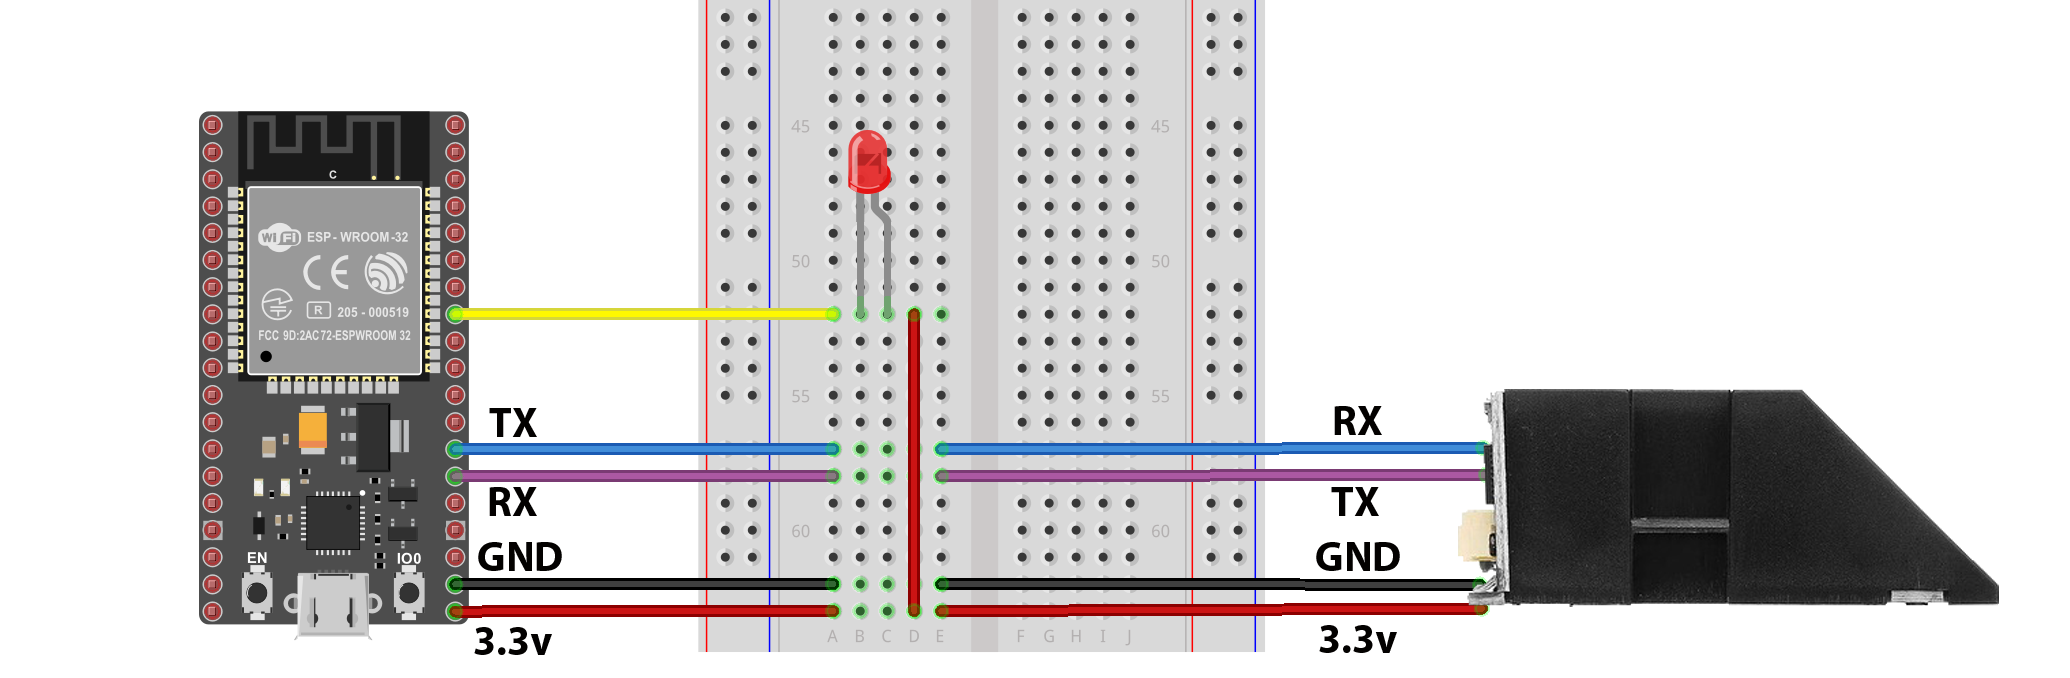
\includegraphics[scale=0.19]{images/schema/montage_illustration.png}
    \caption{Schéma expliquant le montage préliminaire des différents modules  }
    \label{fig52}
\end{figure}

Le schéma ci-dessus révèle la manière dont le module ESP32 Devkit ainsi que le 
capteur d’empreinte DY50 ont été connectés, ainsi qu’une LED pour signaler à 
l’utilisateur la réussite ou l’échec des différentes opérations.

\clearpage  
Branchement: 

\begin{itemize}
    \item [\textbullet]TX (ESP32) -> RX (DY50)
    \item [\textbullet]RX (ESP32) -> TX (DY50)
    \item [\textbullet]GND (ESP32) -> GND (DY50) 
    \item [\textbullet]3.3v (ESP32) -> vcc (DY50)    
\end{itemize}            

Afin d’améliorer l’expérience utilisateur, nous avons rajouté un écran qui 
permettra d’afficher les différents messages comme la réussite ou l’échec 
du pointage ou le nombre d’empreintes enregistrer.

\begin{figure}[h!]
    \centering
    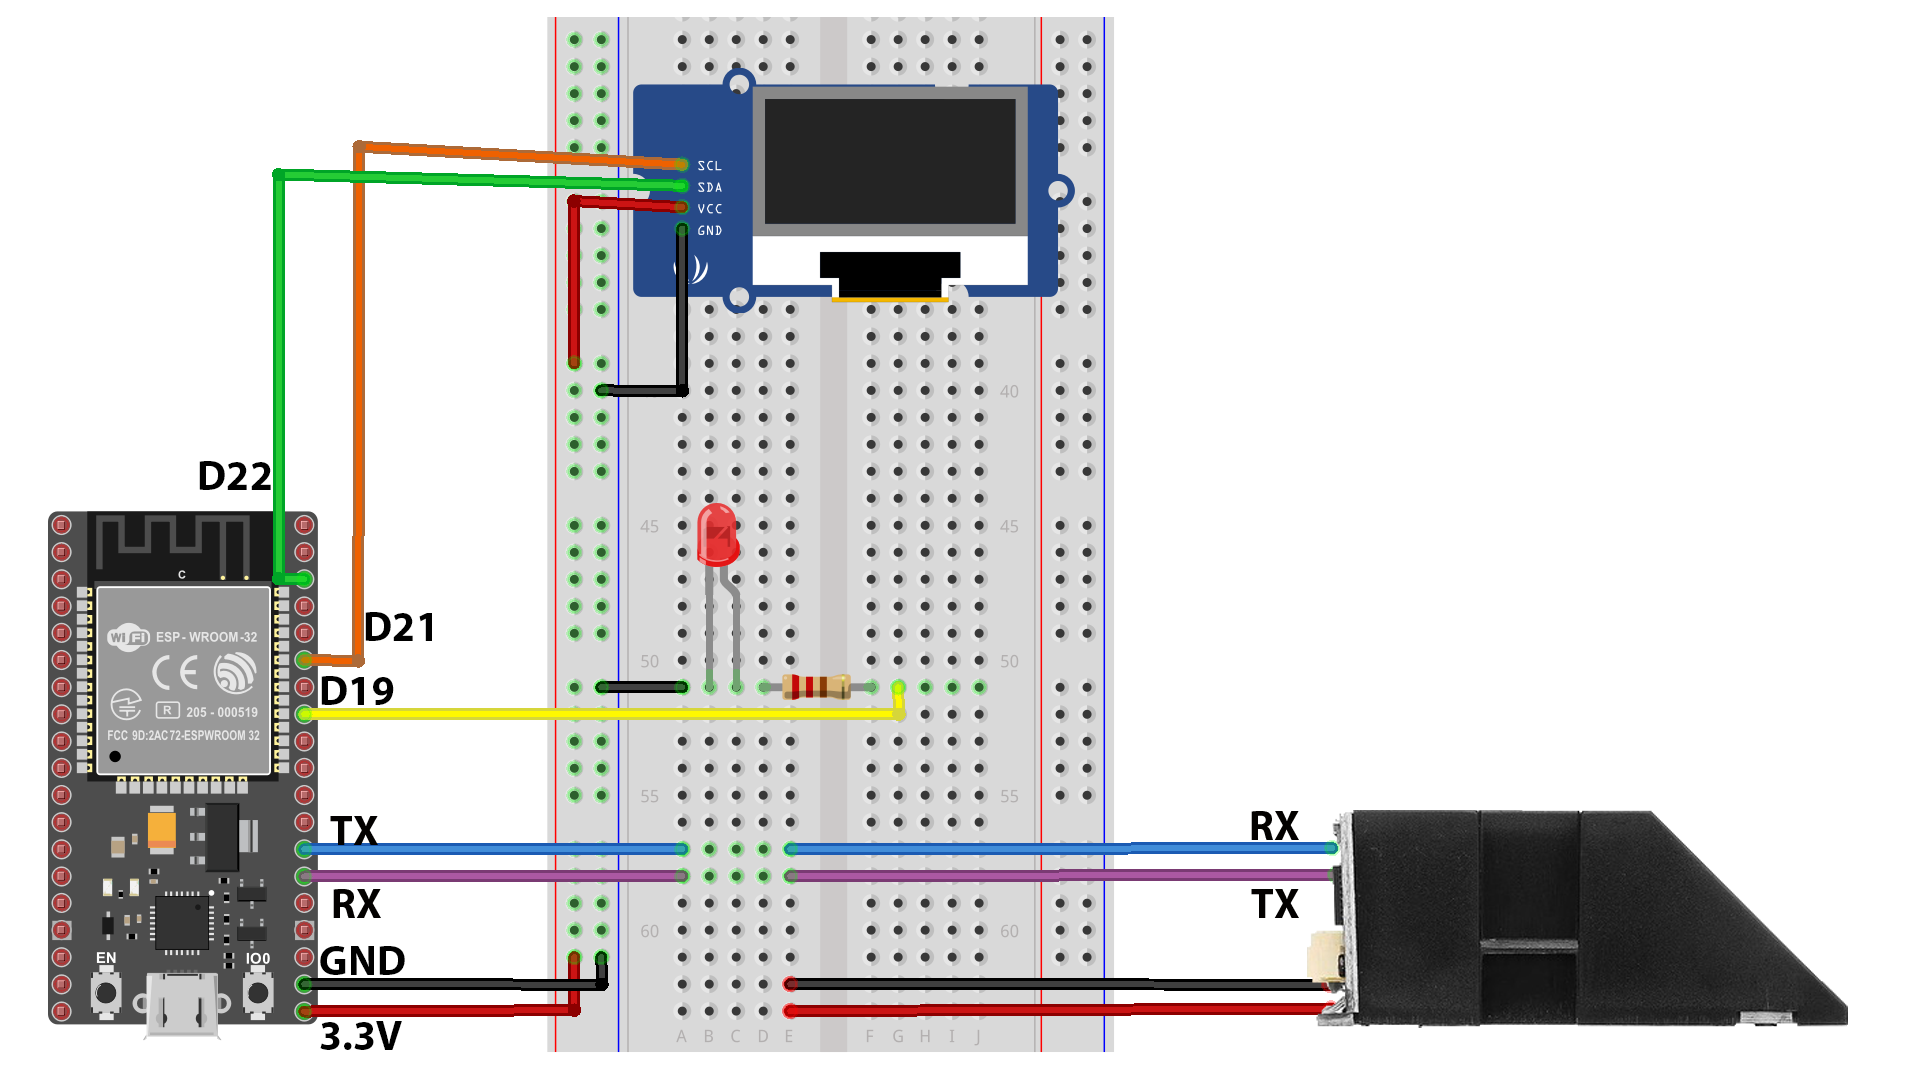
\includegraphics[scale=0.2]{images/schema/schemat v3 sans uvc.png}
    \caption{Schéma expliquant le montage préliminaire des différents modules}
    \label{fig53}
\end{figure}

Branchement: 
\begin{itemize}
    \item [\textbullet]GPIO21 (ESP32) -> SLC (OLED Display)
    \item [\textbullet]GPIO22 (ESP32) -> SDA (OLED Display)
    \item [\textbullet]GND (ESP32) -> GND (OLED Display) 
    \item [\textbullet]3.3v (ESP32) -> VCC (OLED Display)
\end{itemize}    

\begin{figure}[h!]
    \centering
    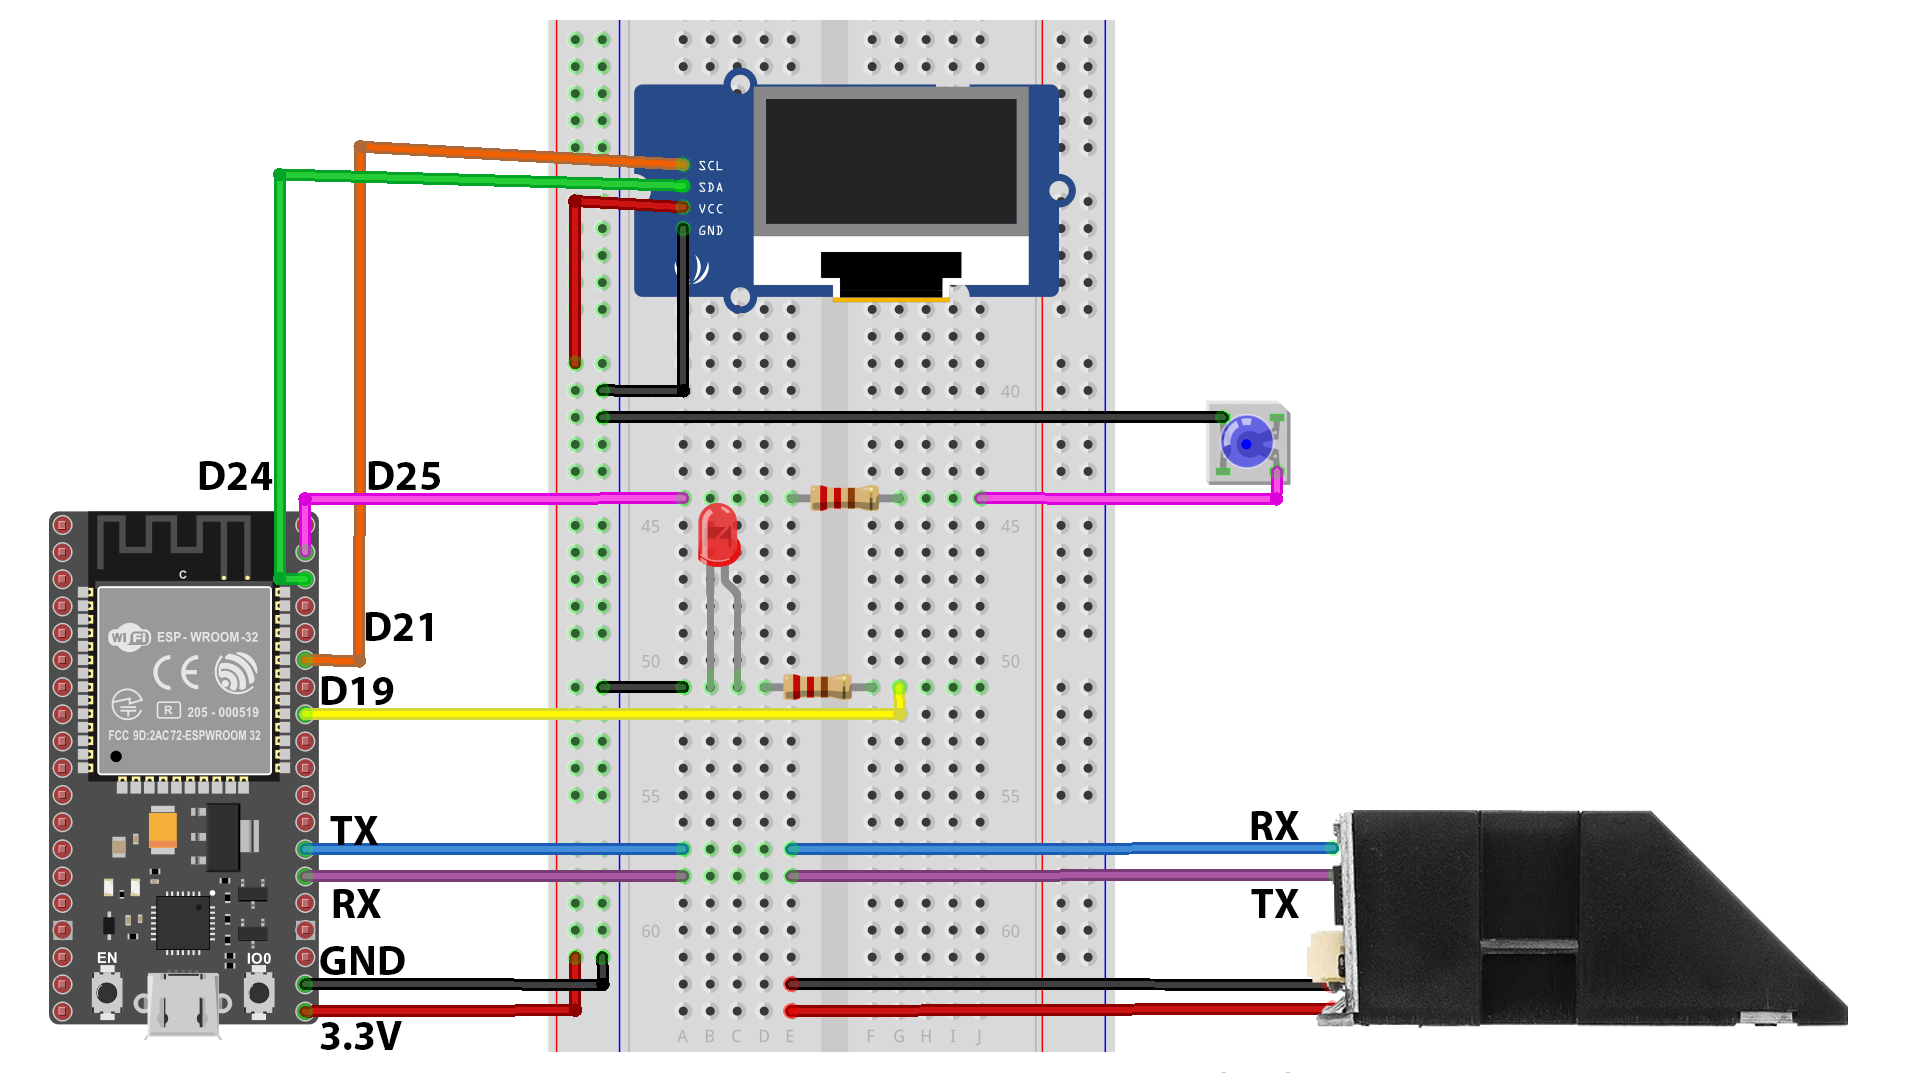
\includegraphics[scale=0.2]{images/schema/schemat_globale.png}
    \caption{Schéma expliquant le montage préliminaire des différents modules}
    \label{fig54}
\end{figure}

Compte tenu du contexte actuel (crise sanitaire due au virus COVID-19) et afin 
de limiter la propagation du virus des gestes barrières sont recommandé. Par 
ailleurs, le fait de toucher une surface ayant était en contact avec plusieurs 
individus sans que cette dernière ne soit désinfectée au préalable constitue un 
risque sanitaire. Pour remédier à ce problème, nous avons décidé d’équiper 
notre pointeuse d’une LED UV-C (lampe germicide). Néanmoins, ce composant doit 
faire l’objet d’une recherche plus approfondie pour confirmer la possibilité 
de l’installer, car la longueur d’onde de ce type de lumière peut avoir des 
effets secondaires indésirables en cas de fortes expositions.

Pour garantir la disponibilité et l’accessibilité du service de pointage, la 
pointeuse doit être fonctionnelle même en cas d’absence de courant. Afin de 
remédier à cette contrainte, nous avons décidé d’inclure une source 
d’alimentation secondaire (batterie) qui alimentera tout le dispositif de 
pointage en cas de coupure de courant ---ceci en supposant que le serveur
hébergeant le système dispose lui aussi d’une alimentation d’urgence en cas de
coupure.    

\section{Prototype}
Le prototype matérialise une étape d’évolution d’un projet, souvent pour
démontrer ou infirmer le bien-fondé d’un ou plusieurs concepts mis en jeu dans
ce projet avant toute valorisation commerciale.

Nous avons décidé de réaliser un prototype en 3D du dispositif de pointage afin 
d’avoir une idée du résultat final.

\clearpage

\begin{figure}[!htb]
    \begin{minipage}{0.5\textwidth}
        \centering
        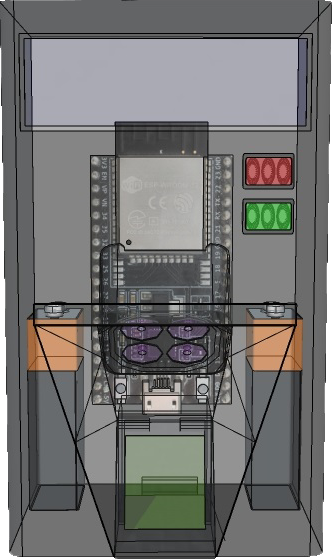
\includegraphics[scale=0.6]{images/prototype/1.png}
        \caption{Pointeuse vue de face}\label{ }
    \end{minipage}\hfill
    \begin{minipage}{0.5\textwidth}
        \centering
        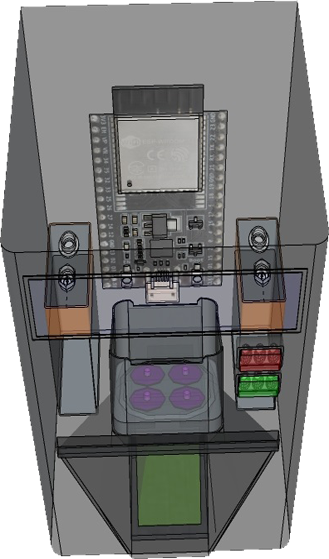
\includegraphics[scale=0.6]{images/prototype/2.png}
        \caption{Pointeuse vue de haut}\label{ }
    \end{minipage}
\end{figure}

\begin{figure}[!htb]
    \begin{minipage}{0.5\textwidth}
        \centering
        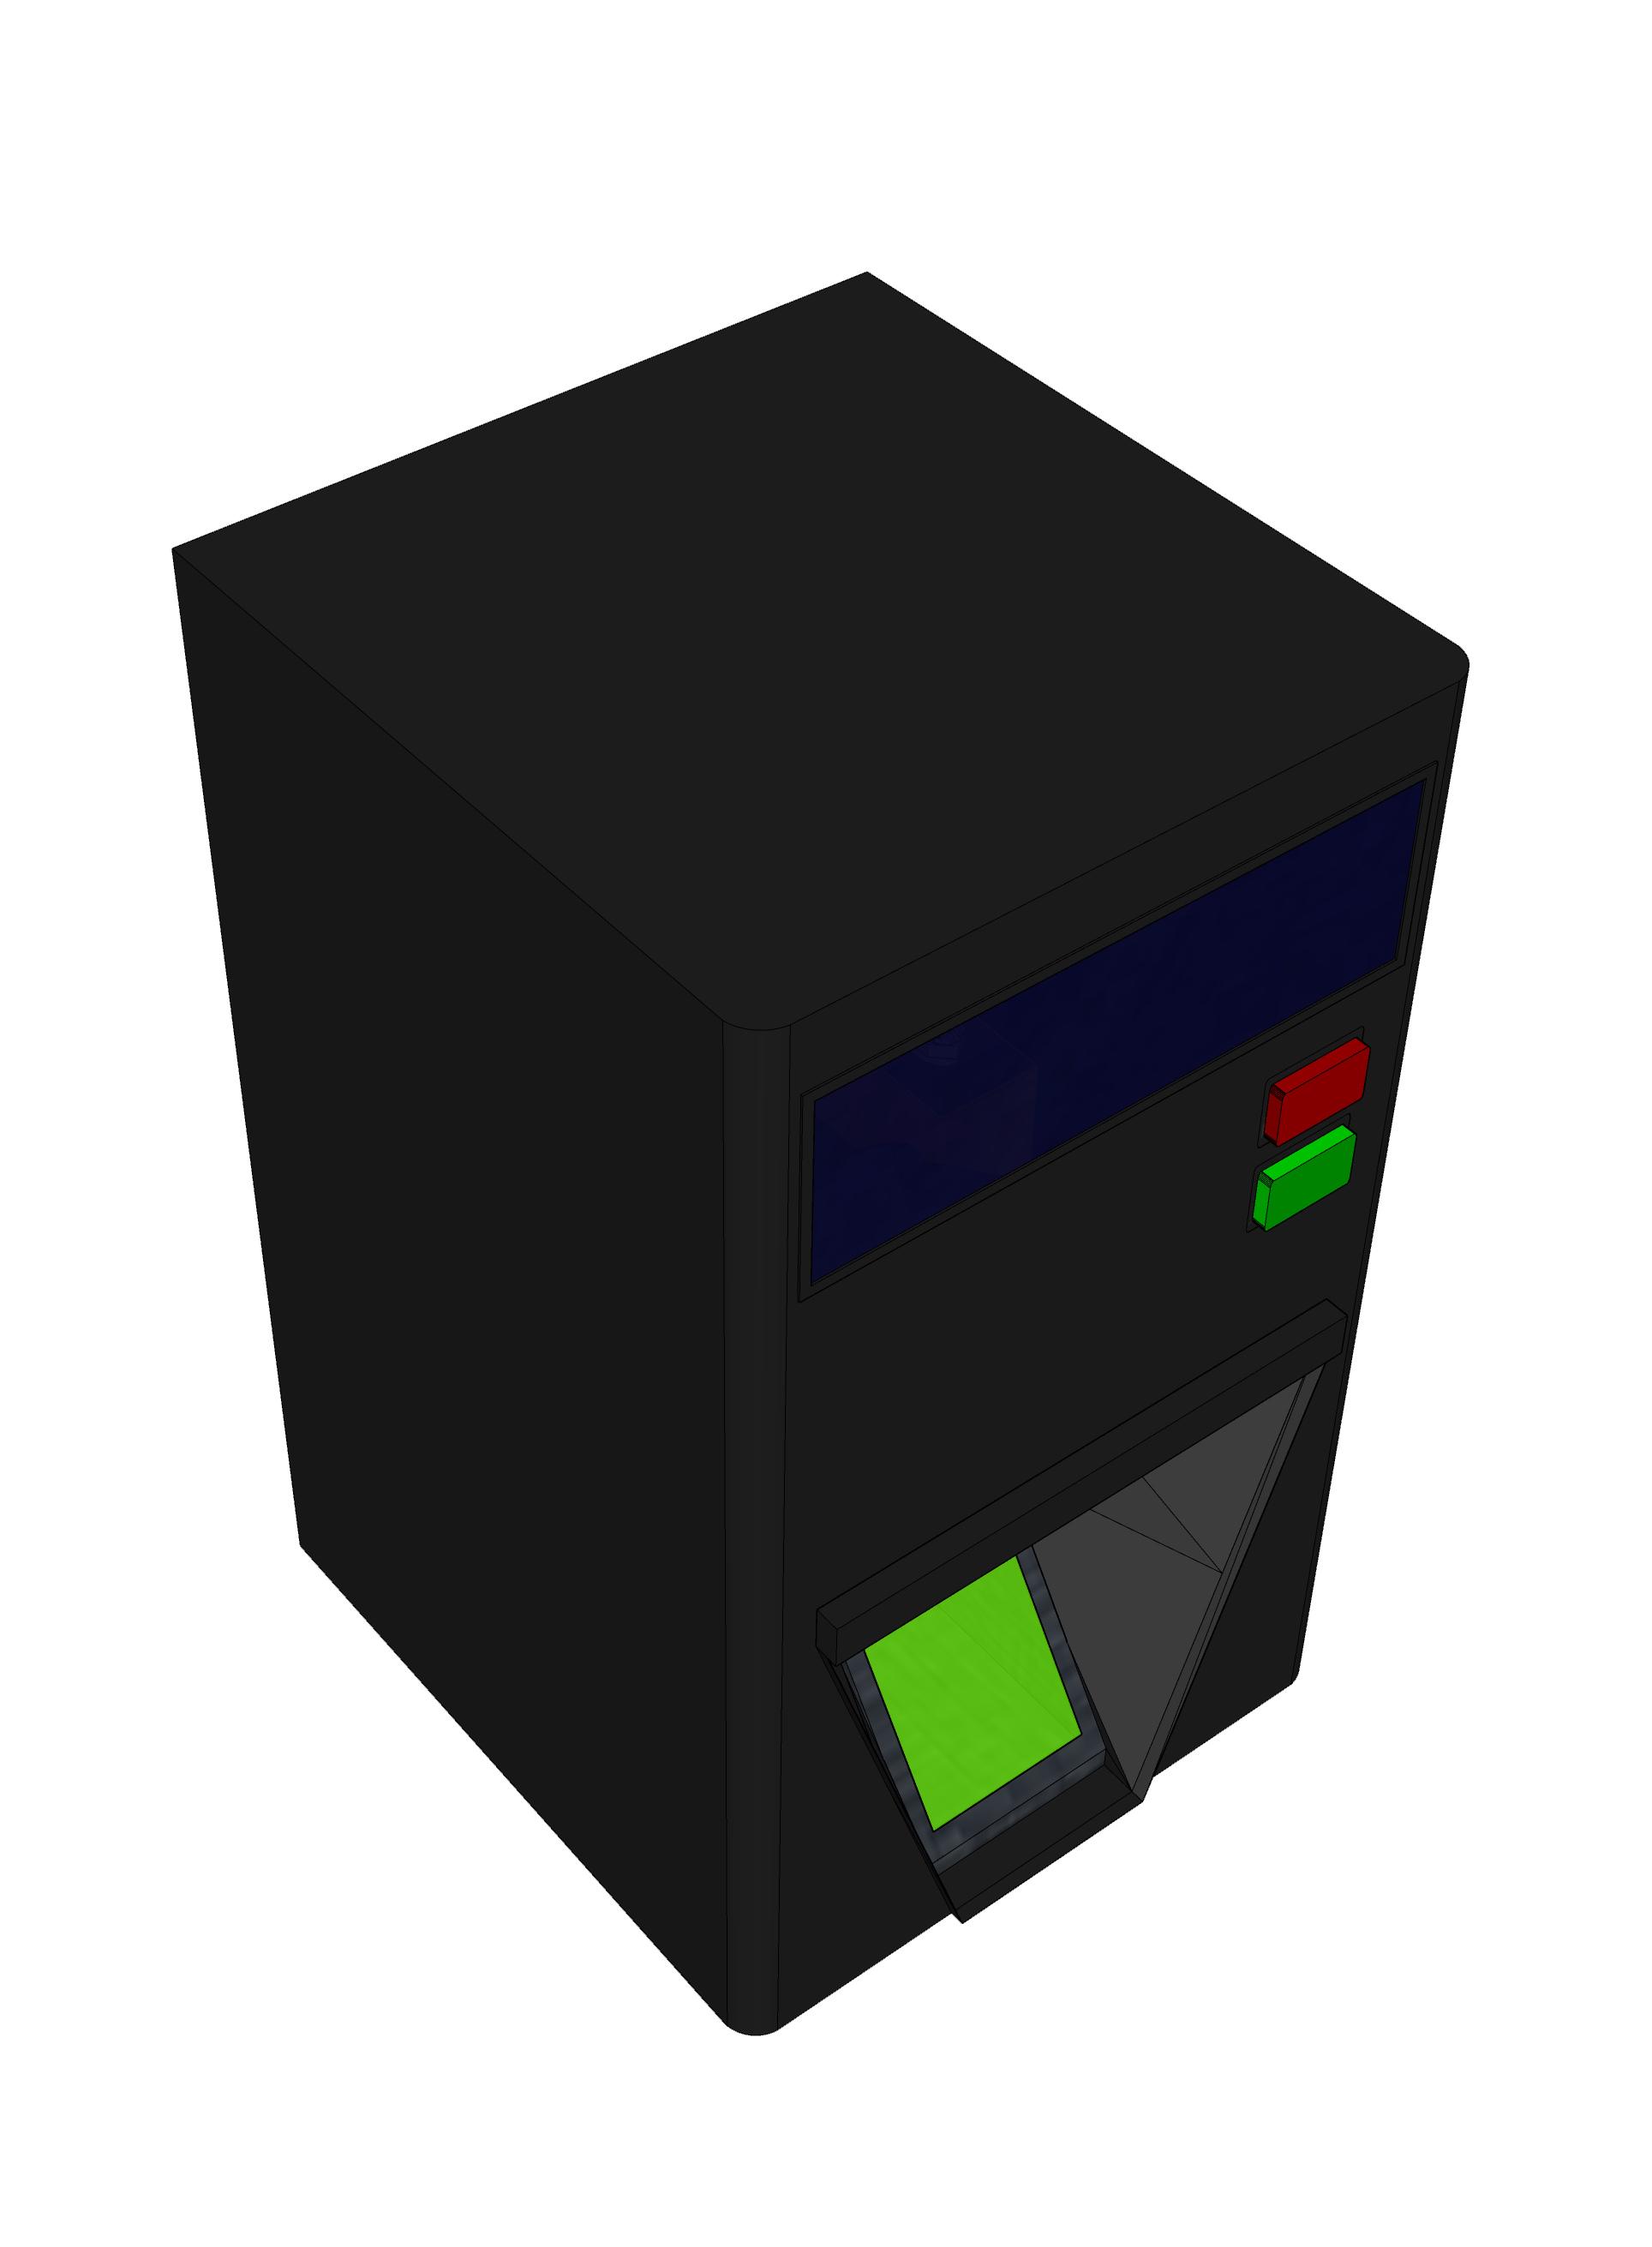
\includegraphics[scale=0.16]{images/prototype/5.png}
        \vspace{-20pt}
        \caption{Côté gauche extérieure}\label{ }
    \end{minipage}\hfill
    \begin{minipage}{0.5\textwidth}
        \centering
        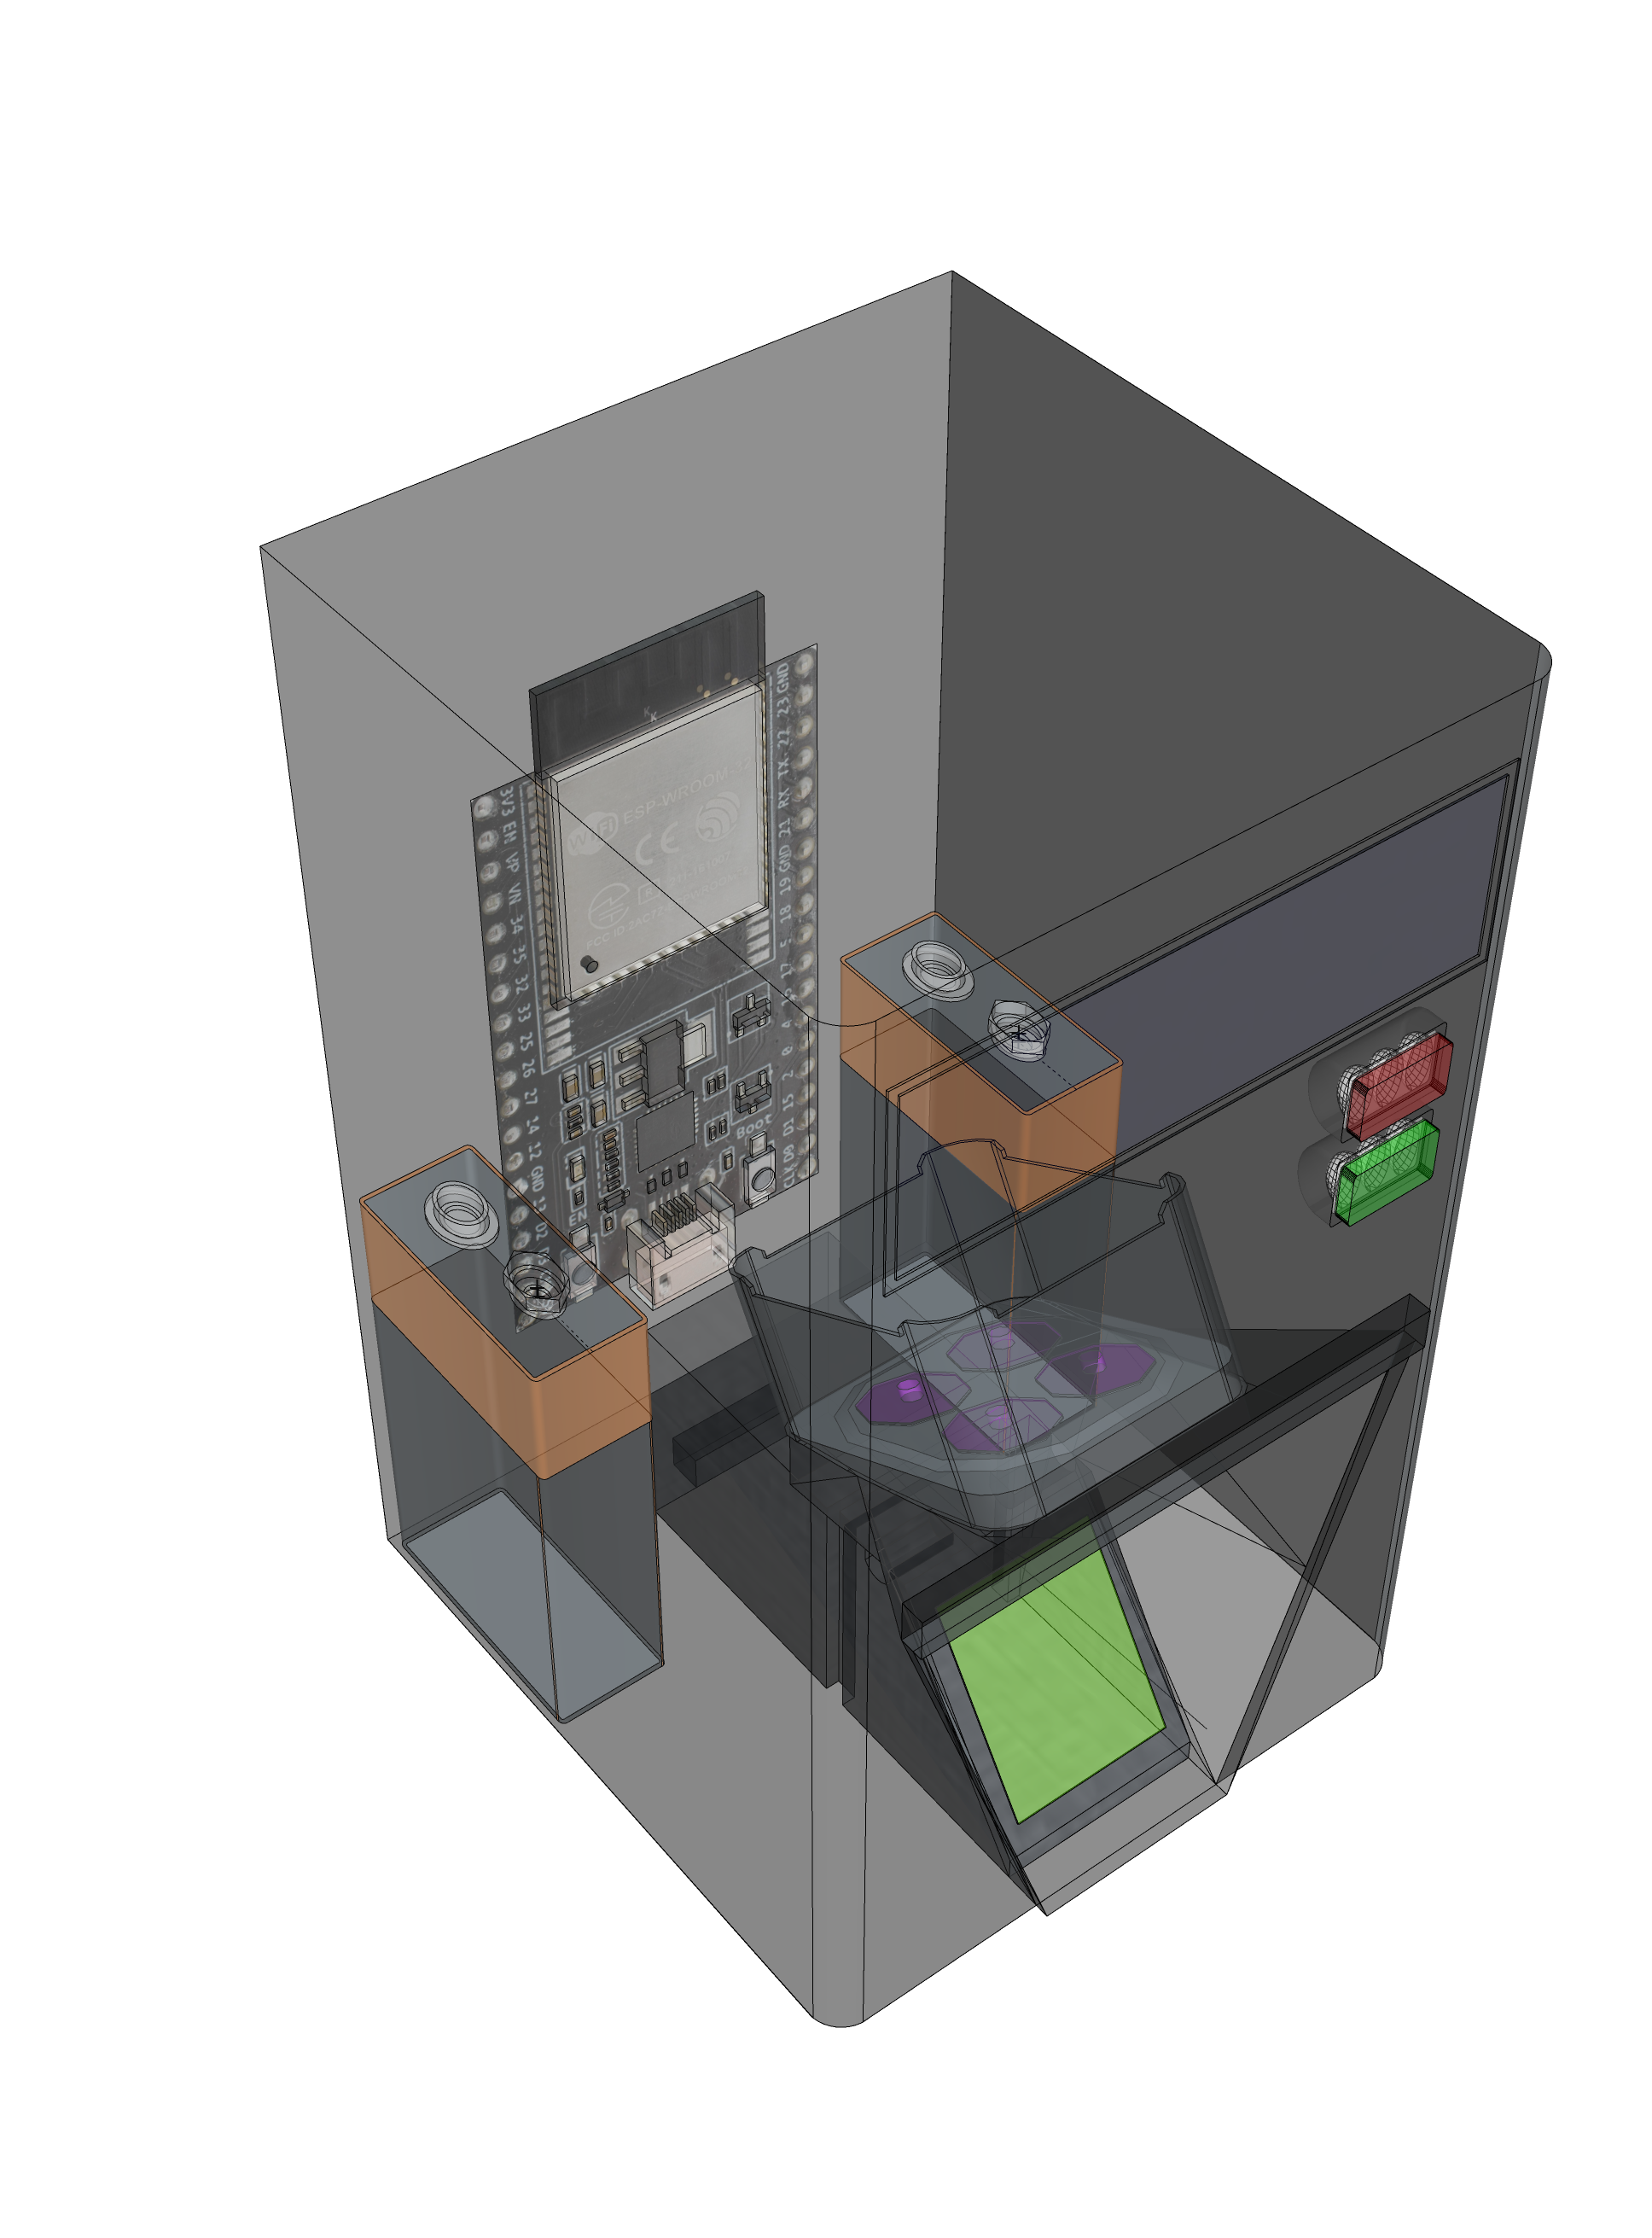
\includegraphics[scale=0.16]{images/prototype/6.png}
        \vspace{-20pt}
        \caption{Côté gauche intérieure}\label{ }
    \end{minipage}
\end{figure}
\clearpage    

\begin{figure}[!htb]
    \vspace{-40pt}
    \begin{minipage}{0.5\textwidth}
        \centering
        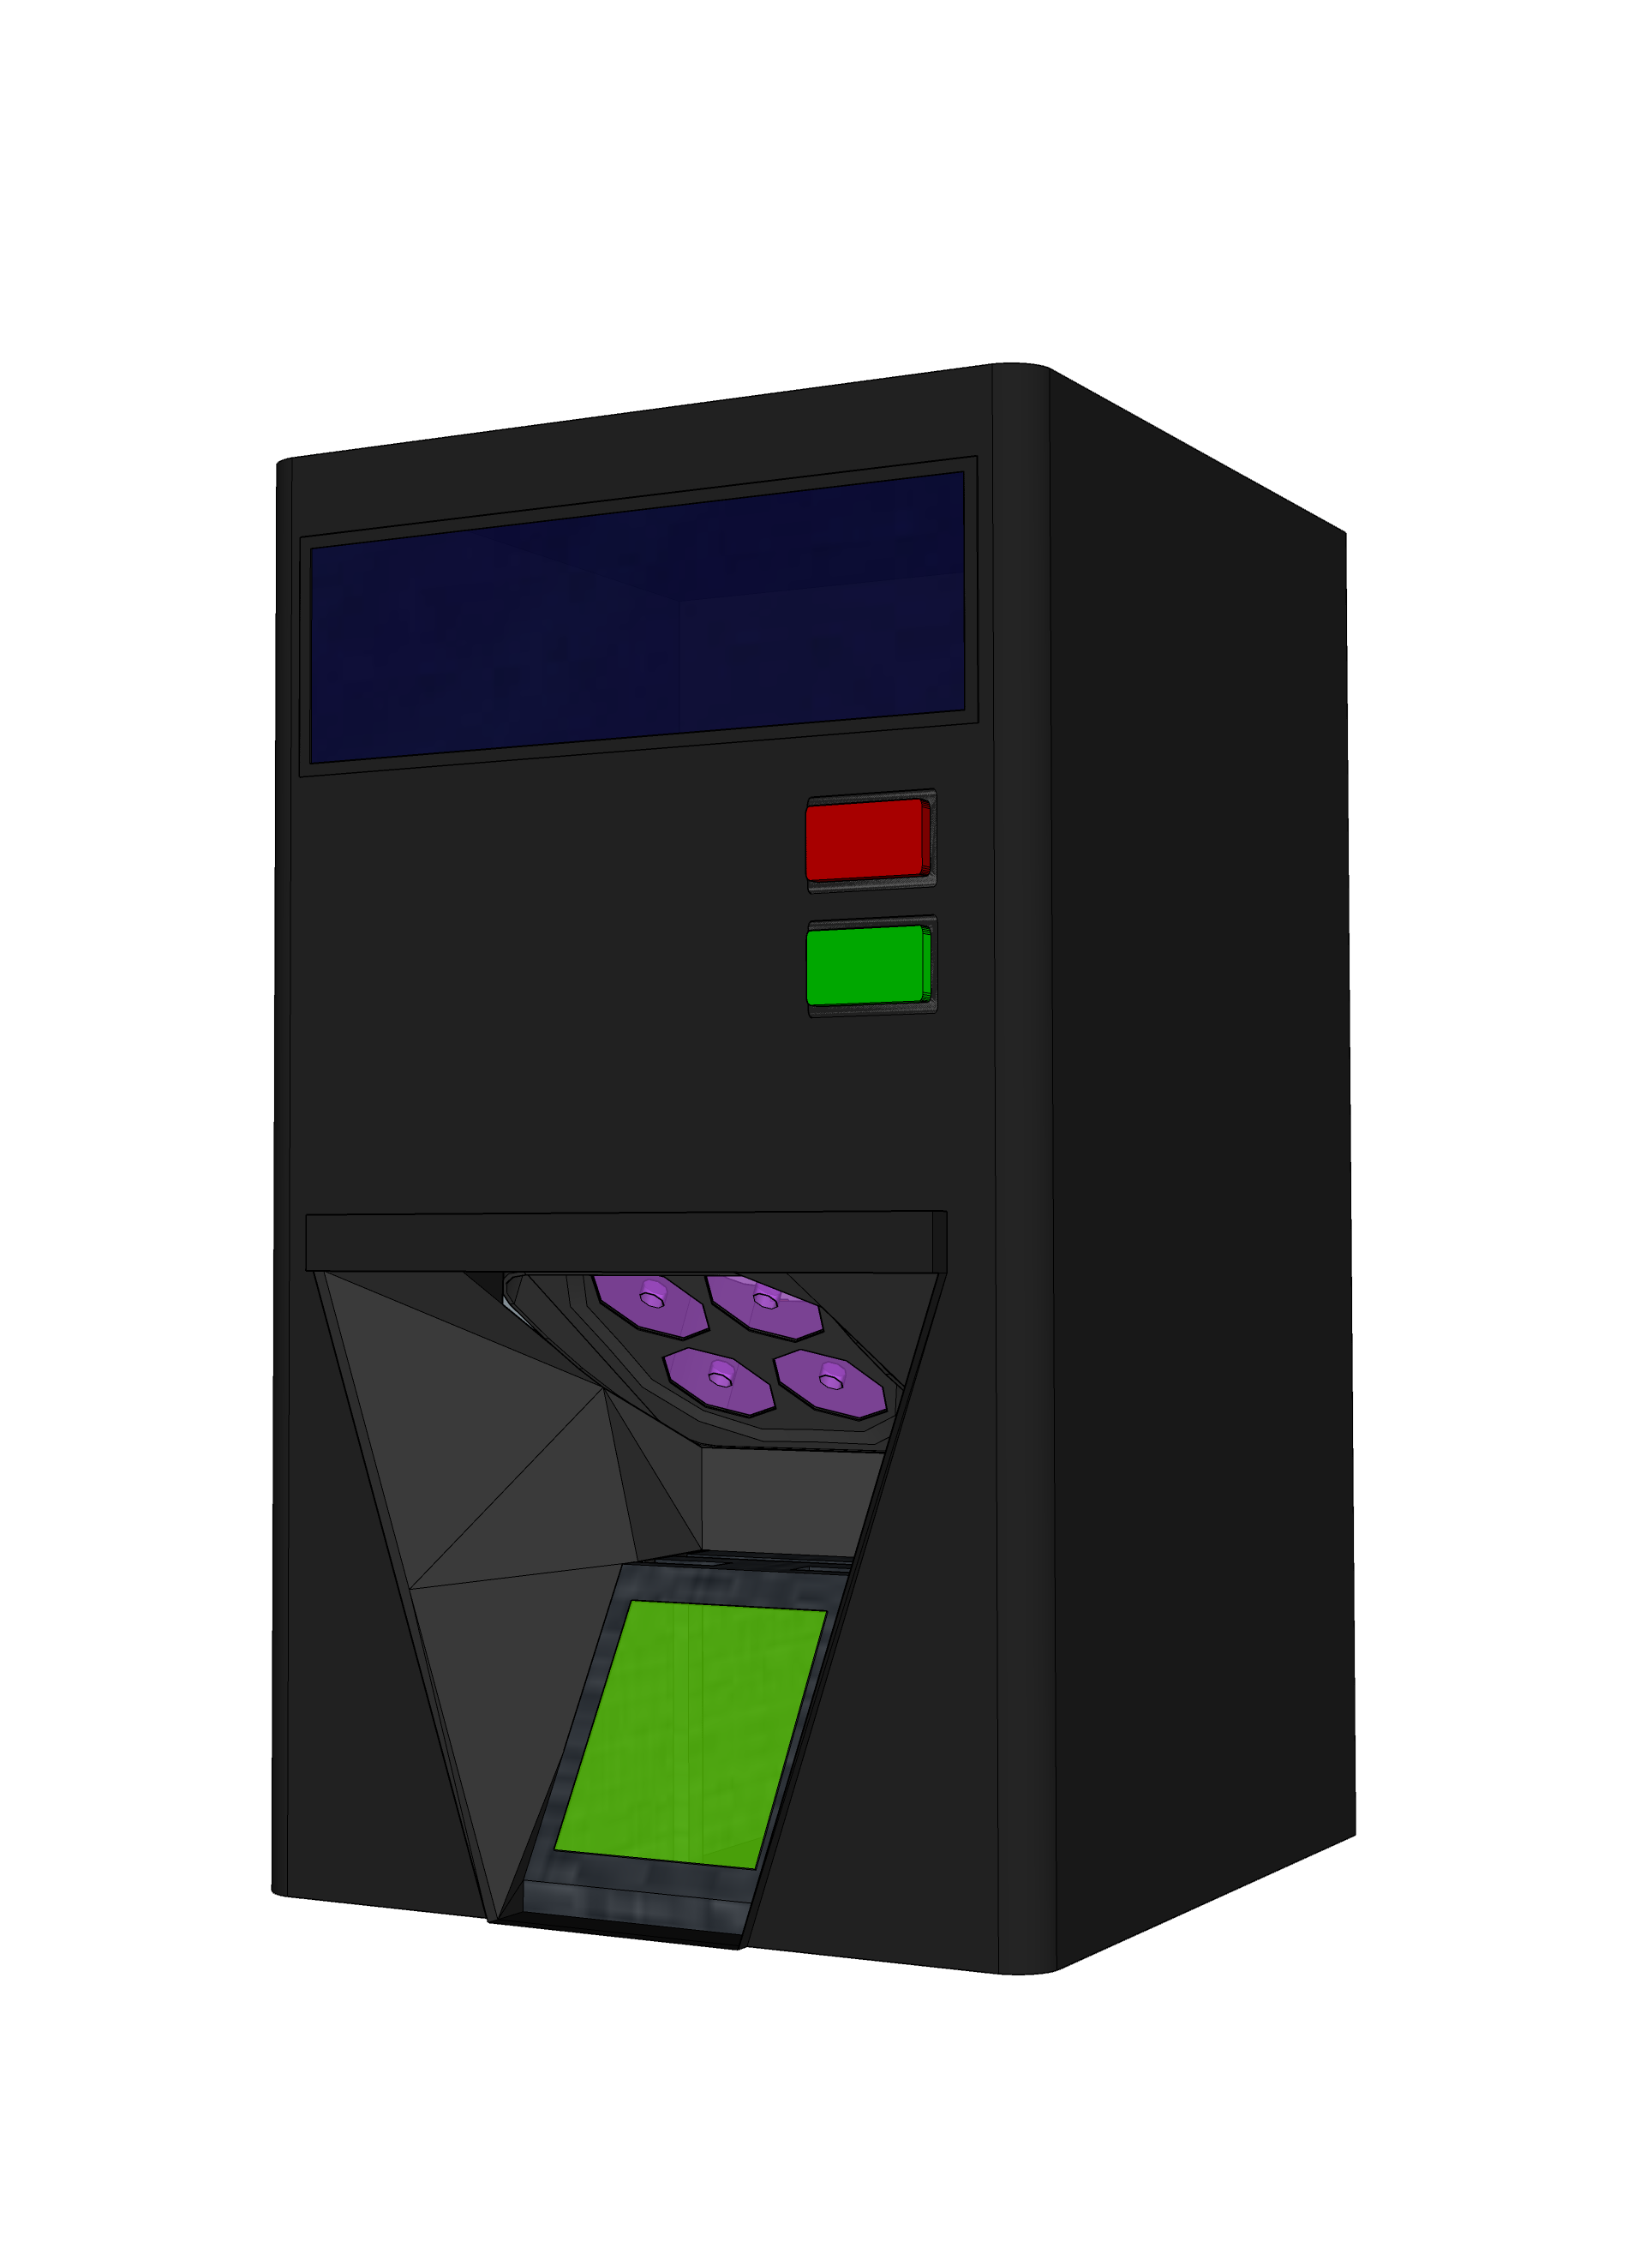
\includegraphics[scale=0.16]{images/prototype/3.png}
        \vspace{-40pt}
        \caption{Pointeuse ouverte}\label{ }
    \end{minipage}\hfill
    \begin{minipage}{0.5\textwidth}
        \centering
        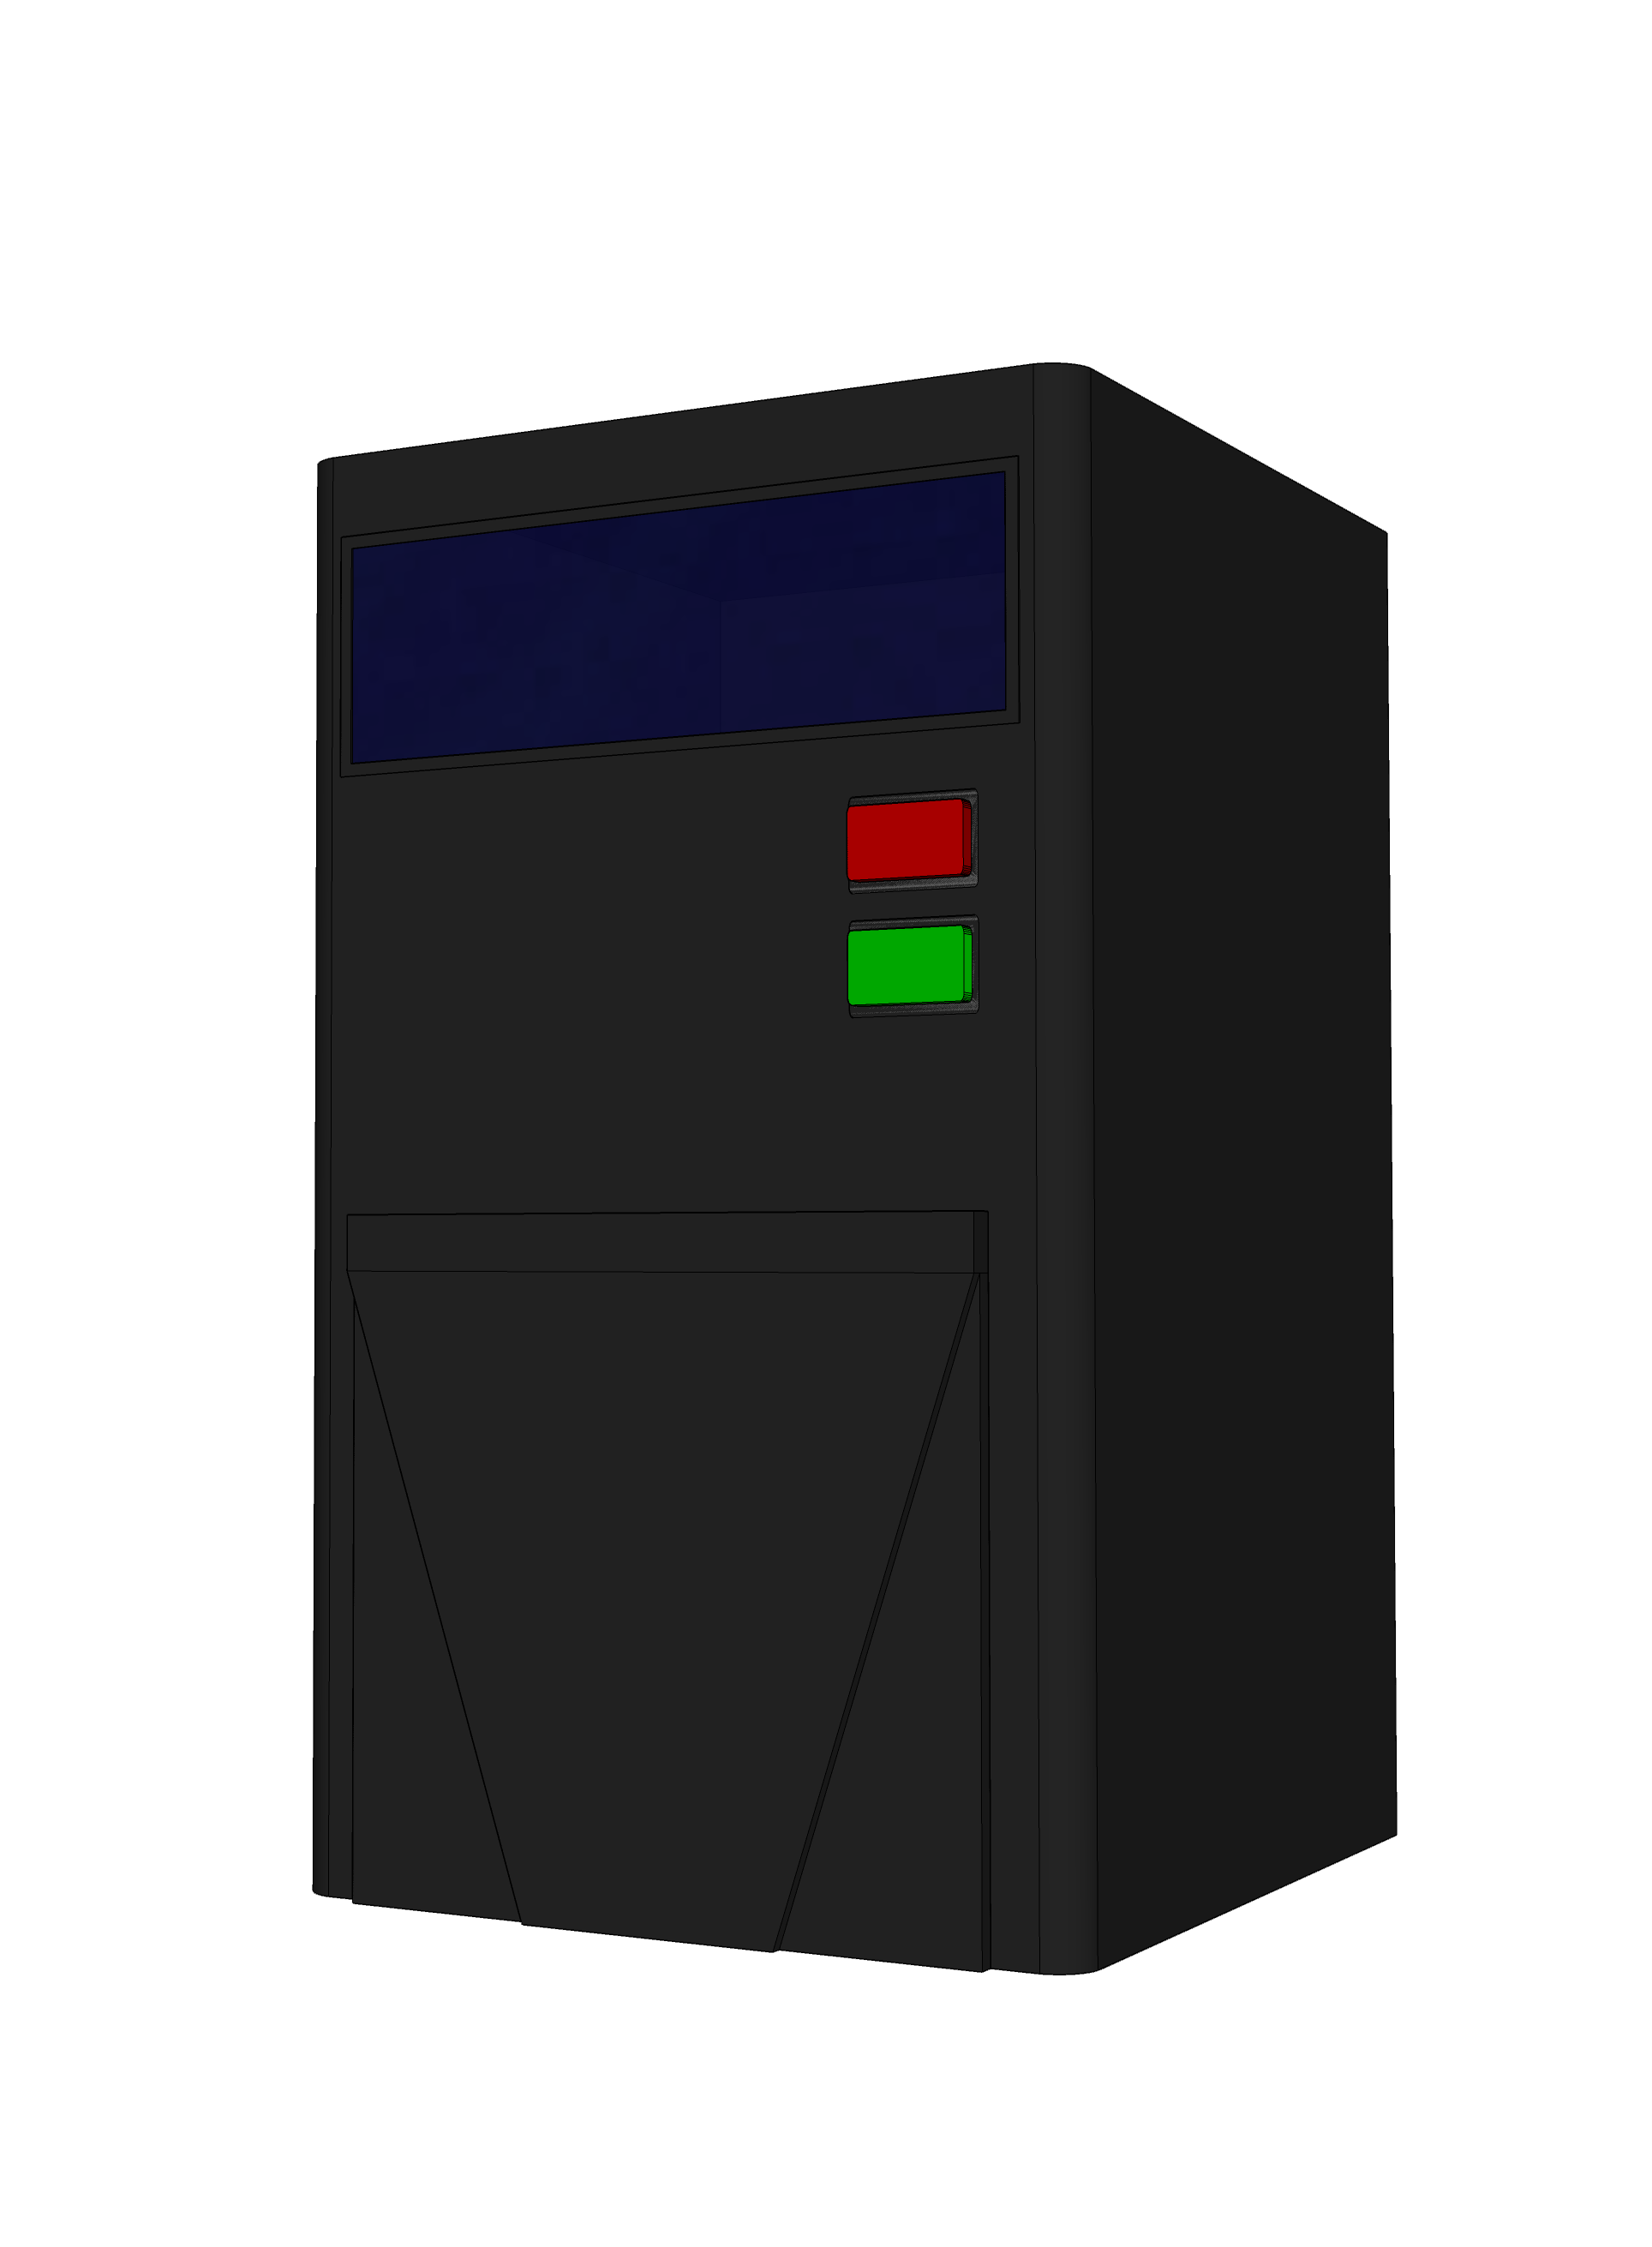
\includegraphics[scale=0.16]{images/prototype/4.png}
        \vspace{-40pt}
        \caption{Pointeuse fermer}\label{ }
    \end{minipage}
\end{figure}

Les images précédentes représentent la disposition des différents composants 
dans un boîtier. Elles nous donnent un aperçu sur l’aspect extérieur de la 
pointeuse et de sa forme. Il est utile de préciser que le lecteur dispose d’un 
cache rétractable, une manœuvre obligatoire lorsque:

\begin{itemize}
    \item [\textbullet] la LED UV-C est utilisée pour désinfecter la surface de
        lecture d’empreinte du capteur. Afin de protéger les utilisateurs des
        effets indésirables des rayonnements ultraviolets.
    \item [\textbullet]  Le dispositif est transporté ou déplacé afin de
        protéger la surface en verre de toute dégradation ou égratignure qui
        pourraient affecter les performances de la pointeuse ou la rendre
        complètement défectueuse.  
\end{itemize}

\section{Programmation}
Une fois les parties matérielles correctement assemblées, nous allons passer à 
la partie programmations de la pointeuse. En premier lieu, nous allons définir 
le rôle de chaque composant ainsi que son champ d’action.

\begin{itemize}
    \item[\textbullet] \textbf{Le module ESP32 DevKit:} Ce dernier représente le
        cerveau de la pointeuse. Car le programme de la pointeuse sera logé en
        lui. Il sera responsable de la communication entre la pointeuse et
        l’application. Il exécutera les différentes commandes exigées par
        l’administrateur (changement de mode
        enregistrement/suppression/pointage, suppression de la base de donnés
        des empreintes au niveau du capteur d’empreinte).  
    \item[\textbullet] \textbf{Le capteur d'empreinte DY50:} Ce dernier
        représente un périphérique d’entrée d’empreinte. À l’aide de sa mémoire
        interne, on pourra sauvegarder les images détaillées des empreintes, ce
        qui minimise drastiquement le temps de reconnaissance des différentes
        empreintes vu que leurs images sont déjà présentes dans la mémoire du
        capteur.

        Comme expliqué précédemment la plateforme Arduino permet de travailler
        avec des modules compatibles, même s’ils sont issus d’un autre
        fabricant. Ce qui est le cas concernant le module ESP32 Devkit et notre
        capteur d’empreintes DY50.  Néanmoins il est indispensable de
        télécharger les pilotes et les librairies des fabricants.    
\end{itemize}

\subsection{Environnement de travail}

\subsubsection{Arduino IDE }
Le logiciel de programmation des cartes Arduino est une application Java libre 
et multiplateforme, servant d'éditeur de code et de compilateur qui peut 
transférer le programme au travers de la liaison série (RS-232, Bluetooth ou USB 
selon le module). Il est également possible de se passer de l'interface Arduino, 
et de compiler les programmes via l'interface en ligne de commande.

\begin{figure}[h!]
    \centering
    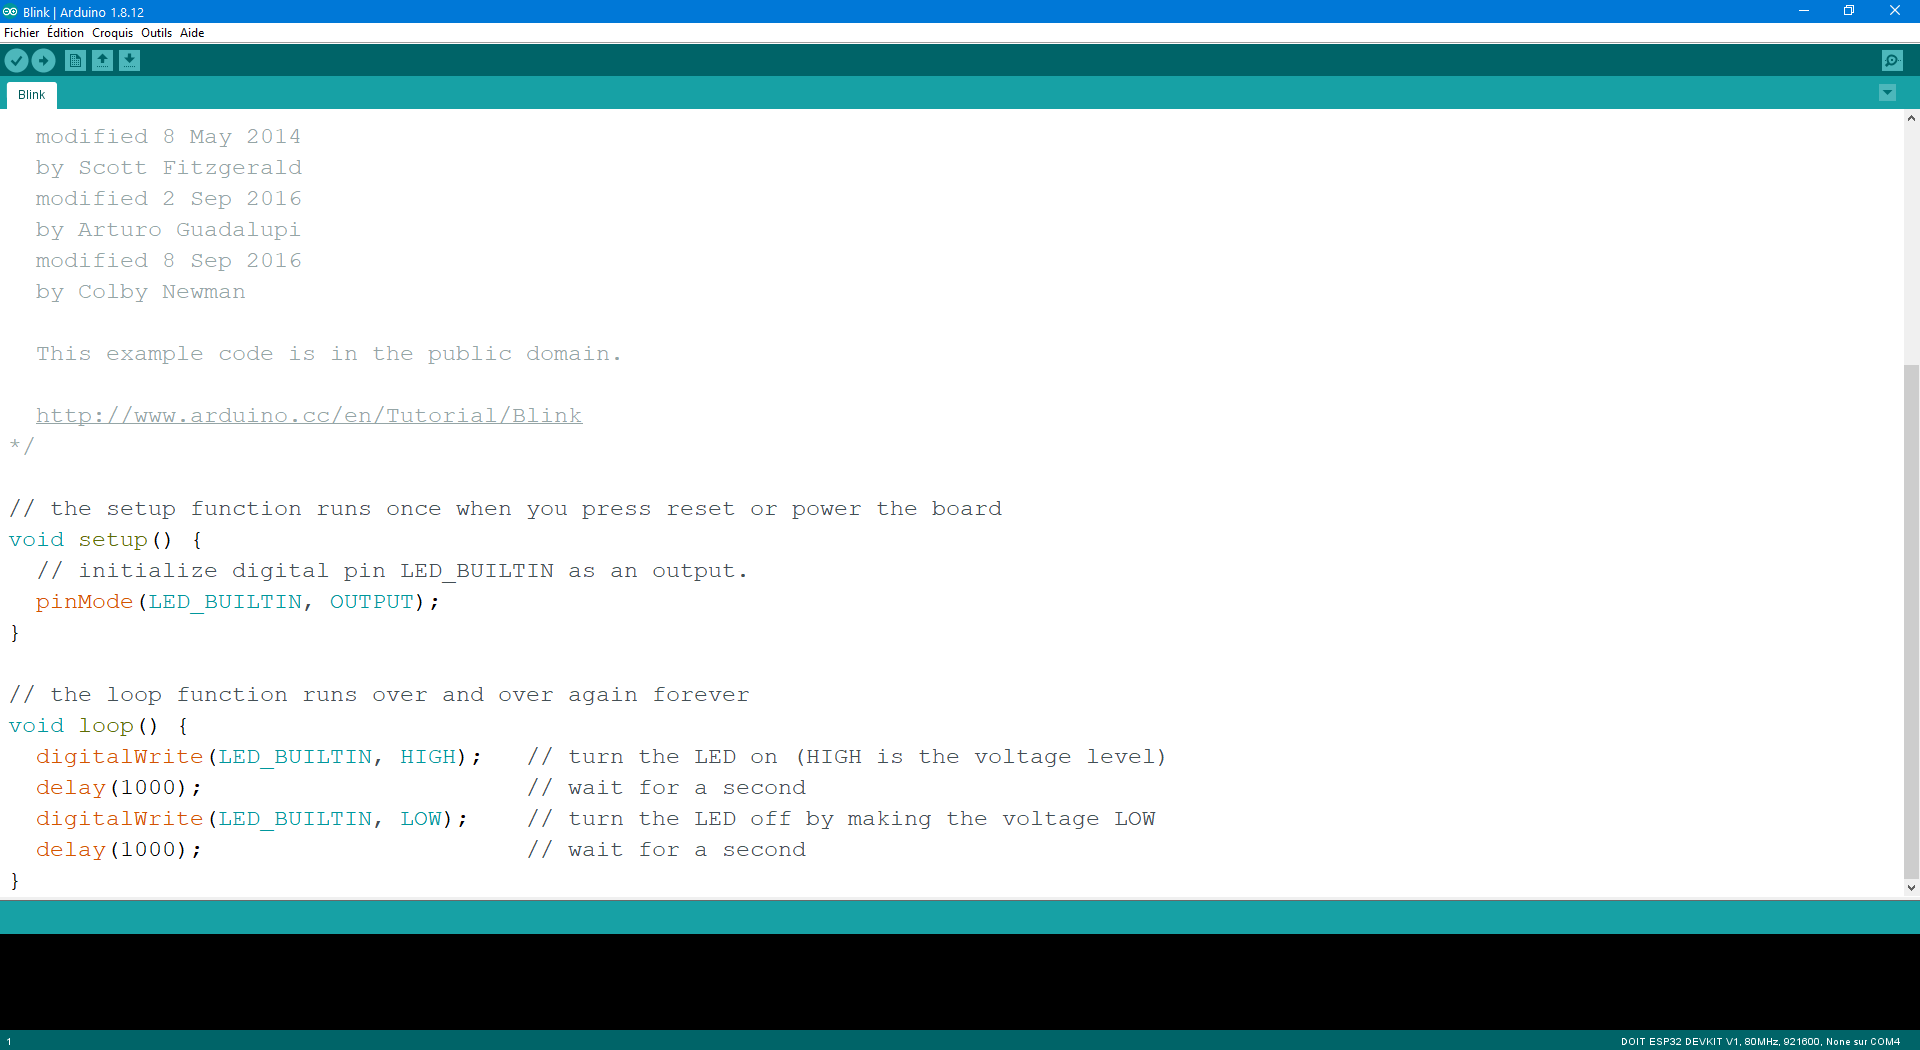
\includegraphics[scale=0.3]{images/arduino_ide.PNG}
    \caption{interface Arduino IDE et un programme qui clignote une LED}
    \label{fig61}
\end{figure}

\subsubsection{Langage de programmation C}
le C est un langage de programmation impératif généraliste de bas niveau. Inventé 
au début des années 1970 pour réécrire UNIX. C’est devenu un des langages les 
plus utilisés, encore de nos jours. De nombreux langages plus modernes comme 
C++, C#, Java et PHP ou JavaScript ont repris une syntaxe similaire et 
reprennent en partie sa logique. Il offre aux développeurs une marge de contrôle 
importante sur la machine (notamment sur la gestion de la mémoire) et est de ce 
fait utilisé pour réaliser les « fondations » (compilateurs, interpréteurs…) de 
ces langages plus modernes.

Ces caractéristiques en font un langage privilégié quand on cherche à maîtriser 
les ressources matérielles utilisées, le langage machine et les données binaires 
générées par les compilateurs étant relativement prévisibles. Ce langage est 
donc extrêmement utilisé dans des domaines comme la programmation embarquée sur 
microcontrôleurs, les calculs intensifs, l’écriture de systèmes d’exploitation 
et les modules où la rapidité de traitement est importante. Il constitue une 
bonne alternative au langage d’assemblage dans ces domaines, avec les avantages 
d’une syntaxe plus expressive et de la portabilité du code source. Le langage C 
a été inventé pour écrire le système d’exploitation UNIX, et reste utilisé pour 
la programmation système. Ainsi, le noyau de grands systèmes d’exploitation comme 
Windows et Linux sont développés en grande partie en C.

En contrepartie, la mise au point de programmes en C, surtout s’ils utilisent 
des structures de données complexes, est plus difficile qu’avec des langages de 
plus haut niveau. En effet, dans un souci de performance, le langage C impose à 
l’utilisateur de programmer certains traitements (libération de la mémoire, 
vérification de la validité des indices sur les tableaux…) qui sont pris en 
charge automatiquement dans les langages de haut niveau\cite{35}.

\subsubsection{esspresif/arduino-esp32 library}
Une librairie écrite et maintenue par le constructeur ESSPRISIF. Cette dernière 
doit être installée au niveau de l'IDE Arduino pour pouvoir téléverser les 
programmes écrits sur le module ESP32 Devkit. Elle est disponible sur: 
<https://github.com/espressif/arduino-esp32>

\subsubsection{Adafruit fingerprint sensor library}
Pour pouvoir interagir avec le capteur d'empreinte cette librairie est 
nécessaire, car elle implémente les différentes méthodes et fonctions qui 
régissent le fonctionnement de capteur d'empreinte DY50 on peut citer:

\begin{itemize}
    \item[\textbullet] check\_model(): qui vérifie le statut du capteur
        d'empreinte. Retourne l'erreur ou OK.
    \item[\textbullet] count\_template(): qui demande au capteur de compter le
        nombre d'empreintes dans sa mémoire et stocker cette valeur dans
        \emph{self.template\_count}.
    \item[\textbullet] creat\_model(): qui demande au capteur de transformer
        l'empreinte en un modèle exploitable. Renvoie le code d'erreur du packet
        ou OK.
    \item[\textbullet] delet\_model(localisation): qui demande au capteur de
        supprimer un modèle d'empreinte de la mémoire flash apres l'avoir
        sélectionné grâce à l'argument 'localisation'. Retourne l'erreur ou OK.
    \item[\textbullet] empety\_librery(): qui demande au capteur de
        réinitialiser toute la mémoire flash ainsi qeu de supprimer tous les
        modèles précédemment enregistrer. 
    \item[\textbullet] get\_image(): qui demande au capteur de capturer une
        image et de l'enregistrer dans la mémoire. Retourne l'erreur ou OK. 
    \item[\textbullet] finger\_search(): qui demande au capteur de chercher
        l'empreinte correspondante à partir du slot 1, enregistre la
        localisation et le taux de correspondance dans \emph{in self.finger\_id}
        et \emph{self.confidence}. Renvois l'erreur ou Ok.\cite{36}
\end{itemize}

\subsection{Code et fonctionnement}    
Comme la plupart des programmes destinés ont des modules qui sont compatibles
avec Arduino, le programme à téléverser est constitué de: 

\begin{itemize}
    \item [\textbullet] une partie pour déclarations des librairies utilisées et
        des variables globales
\end{itemize}

\begin{minted}{c}
    #include <Adafruit_Fingerprint.h>
    #include <HardwareSerial.h>
    #include <WiFi.h>
    #include <HTTPClient.h>

    const char *ssid = "TP-LINK_9C42F4";
    const char *password = "********";
    // post array that will be send to the website
    String postData;    
    //computer IP or the server domain 
    String linkee = "http://192.168.1.222:8000/pointage/getid"; 
    // The Fingerprint ID from the scanner
    uint8_t id; 

    Adafruit_Fingerprint finger = Adafruit_Fingerprint(&Serial2);
    int FingerID = 0;
\end{minted}

le code précédent représente la partie déclarative de notre programme où nous
avons inclus les librairies nécessaires (<Adafruit\_Fingerprint.h>,
<HardwareSerial.h>, <WiFi.h>, <HTTPClient.h>) au fonctionnement de la pointeuse
ainsi que les variables globales utilisées (postData, postData, linkee, id).

\begin{itemize}
    \item [\textbullet] une partie void setup(): qui ne s’exécute qu’une seule
        fois est la partie où nous initialisons et configurons nos
        entrées/sorties et variables 
\end{itemize}    

\begin{minted}{c}
    void setup(){
        pinMode(2, OUTPUT);
        Serial.begin(115200);
        connectToWiFi();

        // set the data rate for the sensor serial port
        finger.begin(57600);
        Serial.println("\n\nAdafruit finger detect test");

        //------------*test the connection*------------
        if (finger.verifyPassword()){
            Serial.println("Found fingerprint sensor!");
        }else{
            Serial.println("Did not find fingerprint sensor:(");
            while (1)
            {
                delay(1);
            }
        }
        //---------------------------------------------
        finger.getTemplateCount();
        Serial.print("Sensor contains ");
        Serial.print(finger.templateCount);
        Serial.println(" templates");

        //SendFingerprintID( FingerID );
        //-------------* deleting all templates"-----------
        //emptyDataBase();

    }
\end{minted}

Dans cette section du code, nous avons initialisé la fréquence de transmission
des différents modules. Ouvrir une connexion au point d’accès déclaré
précédemment, tester la liaison entre l’ESP32 et le capteur, et afficher le
nombre d’empreintes enregistrer dans le capteur (lors de la phase de test).      

\begin{itemize}
    \item [\textbullet] une partie void loop(): est la partie principale où se
        déroule le programme. Tout ce qui va être écrit dans cette zone sera
        exécuté par la carte en boucle. 
\end{itemize}

\begin{minted}{c}
    void loop(){
        //check if there's a connection to WiFi or not
        if (WiFi.status() != WL_CONNECTED){
            connectToWiFi();
        }
        //The ID start form 1 to 127
        // Get the Fingerprint ID from the Scanner
        FingerID = getFingerprintID(); 
        //don't need to run this at full speed.
        Serial.println(FingerID);
        delay(50);
        checkfinger();
        if (FingerID == 1){
            Serial.println("mode Enregistrement/Suppression ");
            checkToDelete();
            delay(5000);
            checkToAdd();
        }
    }
\end{minted}

Cette partie qui sera exécutée en boucle, englobe le comportement que va adopter
la pointeuse une fois en service. Une fois la connexion au point d’accès établie
et le capteur correctement connecté.

\begin{itemize}
    \item[\textbullet] une partie pour les différentes procédures et méthodes
        utiliser 
\end{itemize}

\begin{minted}{c}
    void checkToAdd(){
        HTTPClient http; //Declare object of class HTTPClient
        //Post Data
        // Add the Fingerprint ID to the Post array in order to send it 
        postData = "Get_Fingerid=get_id"; 
        // Post methode
        //initiate HTTP  request, put your Website URL or Your Computer IP
        http.begin(linkee);                                              
        //Specify content-type header
        http.addHeader("Content-Type", "application/x-www-form-urlencoded"); 

        int httpCode = http.POST(postData); //Send the request
        String payload = http.getString();  //Get the response payload

        if (payload.substring(0, 6) == "add-id"){
            // Serial.println("j’ai reçu une réponse qui contient add id");
            String add_id = payload.substring(6);
            Serial.println(add_id);
            id = add_id.toInt();
            if (id != 0){
                Serial.println("posez votre empreinte ");
                getFingerprintEnroll();
            }
        }
        //Close connection
        http.end(); 
    }
\end{minted}

Cette partie du code représente une des nombreuses fonctions déclarées au niveau
de la quatrième partie de notre programme. La méthode checkToAdd() a pour rôle
de vérifier si une empreinte est en attente d’enregistrement après avoir
consulté la base de données du système. Dans le cas d’une réponse «
add-idN°empreinte » le capteur enclenche le processus d’enregistrement d’une
nouvelle empreinte.

Il existe plusieurs fonctions dans le programme qui sont destinées à la
pointeuse (sendFingerPrintID, confirmAdding, checkFinger, etc.) nous avons
décidé de présenter celle-ci à titre d’exemple.

\section{Conclusion}
Dans ce chapitre, nous avons présenté les différentes phases de la réalisation
de la pointeuse ainsi que les différents composants la constituent et les outils
utilisés. Après avoir brièvement présenté la plateforme Arduino, nous avons
exposé les caractéristiques du module ESP32 Devkit ainsi que du capteur
d’empreinte DY50. Ensuite, nous avons illustré le branchement des différentes
parties. À l’aide du prototype, on a modélisé en 3D la pointeuse.  Maintenant
qu’on peut concrètement identifier chaque individu grâce à son empreinte, on
peut passer à l’étape suivante qui est la réalisation du système responsable
d’exploiter cette information.  
